% Template for PLoS
% Version 1.0 January 2009
%
% To compile to pdf, run:
% latex plos.template
% bibtex plos.template
% latex plos.template
% latex plos.template
% dvipdf plos.template

\documentclass[10pt]{article}

% amsmath package, useful for mathematical formulas
\usepackage{amsmath}
% amssymb package, useful for mathematical symbols
\usepackage{amssymb}

% graphicx package, useful for including eps and pdf graphics
% include graphics with the command \includegraphics
\usepackage{graphicx}

% cite package, to clean up citations in the main text. Do not remove.
\usepackage{cite}

\usepackage{color} 

% Use doublespacing - comment out for single spacing
%\usepackage{setspace} 
%\doublespacing


% Text layout
\topmargin 0.0cm
\oddsidemargin 0.5cm
\evensidemargin 0.5cm
\textwidth 16cm 
\textheight 21cm

% Bold the 'Figure #' in the caption and separate it with a period
% Captions will be left justified
\usepackage[labelfont=bf,labelsep=period,justification=raggedright]{caption}

% Use the PLoS provided bibtex style
\bibliographystyle{plos2009}

% Remove brackets from numbering in List of References
\makeatletter
\renewcommand{\@biblabel}[1]{\quad#1.}
\makeatother


% Leave date blank
\date{}

\pagestyle{myheadings}
%% ** EDIT HERE **


%% ** EDIT HERE **
%% PLEASE INCLUDE ALL MACROS BELOW

%% END MACROS SECTION

\begin{document}

% Title must be 150 characters or less
\begin{flushleft}
{\Large
\textbf{Title}
}
% Insert Author names, affiliations and corresponding author email.
\\
Justin Horowitz$^{1}$, 
James Patton$^{12\ast}$
\\
\bf{1} Bioengineering, University of Illinois at Chicago, Chicago, Illinois, United States
\\
\bf{2} Sensory Motor Performance Program, Rehabilitation Institute of Chicago, Chicago, Illinois, United States
\\
$\ast$ E-mail: pattonj@uic.edu
\end{flushleft}

% Please keep the abstract between 250 and 300 words
\section*{Abstract}


\section*{Introduction}
As machines interact more and more with humans, there is a growing need for a rigorous way to understand what people are trying to do, even if they become disturbed, distracted or influenced by pathology. One can assume that a person who is familiar with a particular task will try to do the same thing each time provided all other conditions are equal. This presumes that what people do is on average what they intended to do and that their goal remains unchanged. However, if there is a disturbance, it is unclear what happens to a person's intentions because action is decoupled from intention. Lacking a means to discern that intention and changes in intention leads to challenges in human machine interactions. Hence a comprehensive method for understanding what someone means to do (rather than what they actually do or claim to have wanted to do) as they interact within uncertain environments will prove useful in any area where a person might be thwarted from their intent such as national security, operation of machinery, athletic and music performance, rehabilitation, human augmentation, and artificial intelligence.

It is important to distinguish our use of the term intent from other groups that consider \textit{motivation}\cite{mcclelland1985motives, rawolle2013relationships}, \textit{cost}\cite{todorov2002optimal, flash1985coordination}, or \textit{goal selection decisions}\cite{ziebart2010modeling}. In typical motor control studies, subjects are motivated to complete the experiment in a timely fashion and are usually explicitly provided targets to be reached. Classification of intent is prevalent in both lower \cite{strausser2011development, hargrove2013robotic} and upper limb\cite{englehart2003robust, young2012improving} prosthetics where hybrid control algorithms select from among a set of actions (walking/standing/flexion/extension/etc). While subjects may be \textit{motivated} to complete experiments with minimal effort/cost and their \textit{goal} may be to reach a target, here we use intent to describe the course of action (i.e., the trajectory of the arm) taken in service of goals and motives and not the goals nor the motives themselves. Particularly of interest is the intended course of action when the actual movement is disturbed and hence no longer matches the intent.

Attempts to deduce motor intent in the past have focused on the assumed spring-like properties of human muscles. Springs produce a force according to their impedance and stretch. By measuring force, impedance, and position, Gomi and Kawato\cite{gomi1997human} were able to deduce stretch and thereby infer the muscle's equilibrium point. Supporters of the so-called $\lambda$ model\cite{feldman1995origin} hypothesized that this equilibrium point represented the intent of a movement. Upon inspection of the equilibrium point as it evolved in time, it was clear that it was highly complex and often not anatomically realizable. Therefore, it could not well-represent the intent of a simple reaching movement. We propose a revised method---intent extraction---that deduces intended trajectory, even in the face of disturbances. This method describes a class of filters that map a disturbance, process, actuator, and realized trajectory to an intended trajectory. In human reaching, the process (a dynamic model of the arm), the actuator (viscoelastic muscles), and the realized trajectory are all readily accessible via measurement and modeling. The underlying framework should be extensible to whole-body movement or even more abstract, psychological processes.

Collectively, the general problem of being able to best extract someone's intent is critical to many fields, and hinges on our understanding of the underlying mechanisms through which control is accomplished. We have excellent models of the mechanical properties of arm and muscle because the physics that describe their gross behavior is so well-understood and the need to determine particular physical parameter values has long been clear. This wealth of previous work provides strong footing for our technique, which in turn should yield valuable information not previously available by other means. In fields where the process and actuators are not yet well-understood, this approach may help to structure the search for them.

Understanding the intent has many benefits, and one may be a better way to understand the composition of discrete movements into their subunits. Recent research has strived to understand the composition of movements intention during both infant development\cite{von1979observations} and stroke recovery\cite{rohrer2004submovements}, distinct straight-line subunits with bell-shaped speed profiles increasingly overlap and blend until, as in healthy adult reaching\cite{woodworth1899accuracy}, they become indistinguishable. Flash and Henis \cite{flash1991arm} demonstrated that despite this apparent blending, cued corrections can only be produced at predictable places within the reach. They also showed that these modifications appear to take place by superimposing additional straight-line subunits onto the original movement. Novak et al. \cite{novak2002use} detected corrective subunits following disturbance during knob turning. These studies show planning and correction in discrete subunits, but did not analyze the actual intent and hence cannot be compared to a known, correct trajectory except in the trivial case that movement is undisturbed. A disturbed trajectory's intention is hidden without proper inversion of the model plan for movement. Here we develop a method to extract intent and gain a clearer understanding of subunits from disturbed motions.

In this paper, we employ bidirectional modeling: we convert intent into movement using a forward model so that we can examine the quality and uncertainty of converting movement to intent by intent extraction. We then explore sensitivity and failure modes using standard model analysis techniques. We also demonstrate the accuracy and utility of this on a preliminary dataset of healthy reaching movements disrupted by occasional, unpredictable disturbances. We hypothesize that this combination allows intent extraction with less uncertainty than the uncertainty naturally inherent in point-to-point reaching. We show that certain factors and measurements are more sensitive than others, and demonstrate the viability of this method for a providing a better understanding of what a person means to do when they move and are disturbed.


% You may title this section "Methods" or "Models". 
% "Models" is not a valid title for PLoS ONE authors. However, PLoS ONE
% authors may use "Analysis" 
\section*{Materials and Methods}
The sections below describe the theoretical method, and then present our evaluations. First, we considered an idealized system using synthetic data that demonstrated the concept and provided an understanding of the computational process. Next we conducted an experiment on humans and the process was then evaluated on human subject data. 

\subsection*{Intent Extraction: Deducing the Desired Trajectory}
We first demonstrate the \textit{intent extraction} approach in human motor control, but we later show that the process is applicable to any controlled process with an invertible highest order plant term. The process begins by presuming a model of the controller. Here, we choose the well-known motion control structure of Shadmehr and Mussa-Ivaldi\cite{shadmehr1994adaptive} where the feedforward aspect of the controller perfectly predicts the plant and linearizes the system through cancellation. Additionally, linear feedback rejects position and velocity error. More complex models can be used without any loss of generality. The equation governing the passive planar dynamics (plant) of musculoskeletal structure is of the form:
\begin{equation}
\underbrace{\overbrace{M(q)\ddot{q}}^{\text{Inertia}}+\overbrace{G(q,\dot{q})}^{\text{Coriolis, Centripal}}}_{\text{Plant}}+E=0
\end{equation}
Where $M$ is the mass matrix, $q$ is the joint angles, $G$ contains both Coriolis and centripetal effects, and $E$ is externally-applied torque that the system might interact with. Dots ($\dot{q}, \ddot{q}$) are used to denote time derivatives of the joint angles. The motion behavior changes with the addition of feedforward and/or feedback controllers:
\begin{equation}
\underbrace{\overbrace{M(q)\ddot{q}}^{\text{Inertia}}+\overbrace{G(q,\dot{q})}^{\text{Coriolis, Centripal}}}_{\text{Plant}}+E=\underbrace{\overbrace{\hat{M}(q_d)\ddot{q}_d}^{\text{Inertia}}+\overbrace{\hat{G}(q_d,\dot{q}_d)}^{\text{Coriolis, Centripal}}+\hat{E}}_{\text{Feedforward Controller}}+\underbrace{K_p(q_d-q)+K_d(\dot{q}_d-\dot{q})}_{\text{Impendance, Feedback Controller}}
\end{equation}
Where a hat ($\hat{ }$) over term indicates the nervous system's best estimate of the planar dynamics, also known as the internal model. This portion of the system serves as an inverse-dynamics feedforward controller that cancels out the dynamics of the arm. If the nervous system has sufficient experience and is expecting $E$, it is included as part of the internal model, $\hat{E}$, otherwise $\hat{E}$ is set to zero. $K_p$ and $K_d$ are the lumped impedance and feedback terms that employ a moving state equilibrium to accomplish the desired trajectory, $q_d$. This $q_d$ signifies the unknown desired trajectory that we seek to discover.

For typical dynamic simulations, in order to determine the trajectory the system (i.e., the forward dynamics problem), this second order differential equation requires standard numerical integration to determine the solution to the initial value problem in time. This first involves algebraic manipulation to solve for $\ddot{q}$, and then integration to determine the state trajectory. The intent extraction approach modifies this method by instead solving for $\ddot{q}_d$:
\begin{equation}
\ddot{q}_d=\hat{M}(q_d)^{-1}\left\{M(q)\ddot{q}+G(q,\dot{q})+E-[\hat{G}(q_d,\dot{q}_d)+\hat{E}+K_p(q_d-q)+K_d(\dot{q}_d-\dot{q})]\right\}
\end{equation}  
$\ddot{q}_d$ can then be integrated to determine the intended state trajectory $q_d(t)$. Provided the model of plant and controller are precise, the initial conditions are available and accurate, the mass matrix estimate $\hat{M}$ is invertible, and the constants are accurate and do not vary, and externally-applied force can be accurately measured, then system yields an accurate estimate of the intent.

It is important to distinguish our intended trajectory, $x_d$, from another variable often considered, the equilibrium point of the muscle actuators. Importantly, this has been claimed to be the intended movement. To consider this, we also generalize our approach to any system with a moving intention that governs the control law. This introduces two additional layers of complexity by separating the plant (arm) into its process (dynamics) and actuator components (muscles) and considering the actuator's equilibrium, $x_e$ (sometimes represented as $\lambda$). The feedforward component must use and share this actuator and hence use the actuator's equilibrium. Without loss of generality, we represent the process $P$ and actuator $A$ as linear (or linearizable) operations in some space, $x$:
\begin{equation}
\underbrace{\overbrace{\sum_{n=1}^N P_nx^{(n)}}^\text{Process}+\overbrace{\sum_{m=1}^M A_m(x-x_e)^{(m)}}^\text{Actuator}}_\text{Plant}+E=0
\end{equation}
The internal model of the process ($\hat{P}$ and $\hat{E}$) predicts system actions, external disturbances, and impedance responses in order to determine $x_e$ that $x$ will track a desired path $x_d$.    
\begin{equation}
\overbrace{\sum_{n=1}^N \hat{P}_n x^{(n)}_d+\hat{E}}^\text{Internal Model}+\overbrace{\sum_{m=1}^M A_m(x_d-x_e)^{(m)}}^\text{Actuator}=0
\end{equation}
We solve this for $x_e$ and substituting into eq 4 gives:
\begin{equation}
\overbrace{\sum_{n=1}^N P_nx^{(n)}}^\text{Process}+E=\overbrace{\sum_{n=1}^N \hat{P}_n x^{(n)}_d+\hat{E}}^\text{Internal Model}+\overbrace{\sum_{m=1}^M A_m (x_d-x)^{(m)}}^\text{Feedback (Actuator)}
\end{equation}

Note $x_e$ vanishes, recovering our familiar model. While a proper choice of $x_e$ is critical to control, our approach does not require a model relating equilibrium and intended trajectory. Note also that the actuator's equilibrium $x_e$ is not the process's equilibrium unless all derivatives of $x_d$ are zero. This upholds Gomi and Kawato's finding that the arm muscles' equilibrium does not represent reaching intent\cite{gomi1997human}.

In summary, if the highest order coefficient of the process $\hat{P}_N$ can be inverted and the impedances can be modeled, it is possible to solve for $x_d^{(N)}$ and integrate for $x_d$ revealing the intended trajectory. This general form reveals the conditions needed to solve for the moving intent of an arbitrary dynamic process. 

\subsection*{Generation of synthetic data using simple dynamic simulation}
We choose one prevailing arm model, that of Burdet et al. \cite{burdet2006stability}, along with the anatomical mass distribution and geometry parameters of Winter \cite{winter2009biomechanics} to create a model for estimating intent. The model of Burdet et al \cite{burdet2006stability} was adapted to reflect measured physical parameters of the subject who provided the reach. Segment lengths were measured directly while gross body mass was self-reported. These values were converted to segment masses, centers of gravity, and moments of inertia inertia using anatomical landmarks and values from Dempster \cite{dempster1955space} and Winter \cite{winter2009biomechanics}. The muscle torque used to calculate stiffness was approximated by looking backward in time a small amount (500 microseconds). Desired trajectory in time was simulated as a minimum jerk, 5th order polynomial of duration 700ms starting and ending with zero velocity and acceleration.
Simulated reaches were 15 cm long, beginning 38 cm out from and 5.7 cm left of the right shoulder then proceeding right.  We used the following types of perturbing forces for each combination of distance and direction: 
Pulse forces applied in one of the the two directions perpendicular to the direction of movement began when the subject had moved either 10\% or 50\% of the distance to the target and lasted for 150ms.
Noise forces began once the subject moved 3 mm, and lasted for the duration of the motion. The forces were drawn from a white noise generator drawn at 1000 Hz with flat power spectral density of 1N, and then passed through a 4th order low-pass Butterworth filter with cutoff $10\pi$ rad/s. 

\subsection*{Error Metric}
Our error metric used deviation in position, where unsigned error was calculated as the mean magnitude of deviation from the nominal trajectory across each of 150 1mm wide bins spaced evenly throughout the 15cm reach.  Mean unsigned error (MUE) was also used to summarize the overall error in each movement for sensitivity analysis. Maximum unsigned error, also called maximum perpendicular distance, was used to measure reaching accuracy to avoid sensitivity to duration of inspection.

\subsection*{Indices of variance-based sensitivity}
Sobol-distributed matrices were generated using MATLAB's sobolset() function and converted to parameter distributions (see Table~\ref{tab:parameters}) using inverse cumulative probability density. Distributions were clamped to the range of $\pm3$ standard deviations in order to avoid support for implausible parameter values. Combinations and calculations were made as prescribed by Saltelli et al. \cite{saltelli2010variance} to arrive at direct and indirect sensitivity indices.

\subsection*{Human Subjects}
The human data trajectories analyzed here are drawn from a four subjects who gave informed consent in accordance with Northwestern University Institutional Review Board. Two male and two female right-handed subjects (ages 24 to 30) performed the reaches with their right arm and was not compensated. Subjects' arm segment lengths were directly measured \textit{in situ} while body mass was self-reported.

\subsection*{Apparatus}
A planar manipulandum (described in Patton and Mussa-Ivaldi \cite{patton2004robot}) was programmed to compensate and minimize any handle friction or mass. The MATLAB XPC-TARGET package (Natick, MA) was used to render this force environment at 1000 Hz and data were collected at 1000 Hz.  Visual feedback was performed at 60 Hz using OpenGL. Closed loop data transmission time (position measurement to completed rendering to recognition of rendering by the position measurement system) was <8 ms, ensuring a visual delay less than one 60 Hz frame.

\subsection*{Protocol}
Subjects made 730 reaches in total, along a line parallel to their coronal plane and approximately 45 cm from their shoulder. Reaches were either 15 or 30 cm long, starting and ending at one of three points spaced 15 cm apart on the line. To prevent any learning effect, forces were presented intermittently with random frequency, but never less than 5 reaches apart. Forces were chosen pseudorandomly such that each type, direction, and distance combination mentioned above was presented 5 times.  

\subsection*{Statistical Analysis}
The MATLAB statistics toolbox package (Natick, MA) was used to perform comparisons among subjects and trajectory sources using the nonparametric Kruskal-Wallis test with Tukey-Kramer post-hoc for group differences. Nonparametric testing was necessary due to floor effects from using unsigned measures.


% Results and Discussion can be combined.
\section*{Results}

\subsection*{Model Viability}
Sensitivity analysis fortunately revealed that variance in intended trajectories due to estimated uncertainty in model parameters is lower than the natural variation in undisturbed motions.  Simulated point-to-point reaches disturbed by either filtered white noise forces or a pulse force perpendicular to the direction of the reach (figure 1) were extracted in the presence of 220,000 variations upon the parameters (table 1) according to the methods of Saltelli et al. \cite{saltelli2010variance}. Expected variation due to parameter uncertainty was 0.86 microns for pulse forces and 1.5 microns for filtered white forces. Variation in recorded undisturbed point-to-point reaching under the same time and reach distance conditions was 2.93 microns. These variations both fall beneath the instantaneous accuracy of the robot recording the motion (tenths of a millimeter). In other words, while some inversion processes might be highly sensitive to model uncertainty, our process for recovering intent from action is much more precise than its input.

\subsection*{Parameter Sensitivity}
Simulated error due to direct parameter uncertainty (figure 2) reached the order of millimeters and revealed particular sensitivity to misestimation of stiffness and changes in shoulder position from trial to trial. Indirect sensitivity, which reveals how errors from other parameters are affected by changes in a given parameter, was an order of magnitude lower than direct sensitivity and again implicated stiffness estimation inaccuracy as a primary cause of extraction uncertainty. Note that this sensitivity analysis does not provide information on whether models or parameter estimates are accurate, only how sensitive the model would be if they were inaccurate. 

\subsection*{Human Intent Trajectories}
Extraction of intent from human point-to-point reaching revealed straight-line movement that persisted for hundreds of milliseconds after the onset of disturbing forces (figure 3). In both pulse timing conditions, intent remained straight line towards the target, supporting the approach.  When disturbances occurred early in reaching, intent showed some signs of correction mid-reach. When disturbances occurred late in reaching, intent tended to continue to onto the target with change of intent occurring on or near the target (figure 3 lower plots). 
Patterns across all trials and subject revealed some systematic tendencies. For approximately 200 milliseconds after the onset of disturbance (figure 4 compare individual points). At this point intent significantly deviated from the baseline region of tendency. As the movement completed, the hand position and intent re-converged and become statistically indistinguishable at approximately 400ms after the onset of disturbance (figure 4 shaded areas).

\section*{Discussion}
We sought to determine the plausibility and robustness of an algorithm that determines a person’s intent of a motion, even if there disturbances. Sensitivity analysis on synthetic data revealed that the method was plausible and response to parameter variations was more robust than human reaching, but significant misestimation could occur if the stiffness was inaccurately modeled. Examination of intended trajectories from force pulse-disturbed human reaching confirmed that these intentions remained statistically indistinguishable from undisturbed reaching for ~100ms following the onset of disturbance. This test provides a method for testing and potentially falsifying our extraction. Differences after this point could be attributed to many factors including unmodeled reflexes, changes in arm stiffness, or genuine change in movement intent. In the context of the sensitivity analysis, it appears most likely that this primarily represents a change in intent and thus a first look at how intent changes when faced with a force disturbance.

$\lambda$ models seek to explain reaching intent as the muscles’ equilibrium trajectory. By deriving the technique in a general form, we discovered that our $x_d$ can be used to determine the muscle equilibrium of a $\lambda$ model and that they are only equivalent when $x_d$ is not changing. Even as this rejects a major claim of those modeling approaches, it explains a key experimental underpinning: Bizzi’s et al.’s \cite{bizzi1984posture} discovery of a “virtual trajectory” in deafferented monkeys with a moving equilibrium point that progressed smoothly from the initial to final positions. Even if the muscle equilibrium jumped abruptly, this would be insufficient to move the intended trajectory abruptly due to the presence of a virtual mass.

Not only is intent slow to change, it does not necessarily change due to disturbance. While this work does not examine this directly, our observations are more compatible with intermittent control (or even submovements) than with continuous optimal feedback control. In classic optimal control, the system is always updating the intent in response to errors \cite{todorov2002optimal}. Our results suggest a latent response consistent with sensory feedback latencies \cite{pruszynski2012optimal}. Interestingly, our data disturbances that come later in the movement appeared to not dramatically affect the intent (Figure 3, lower plot), suggesting that people may stubbornly “stick to their guns” when they know that the stiffness and damping characteristics will provide enough restoring torque to arrive at the target. In other words, response latencies may be  dependent on the time of the disturbance in the movement. Another explanation is that control is intermittent \cite{gawthrop2011intermittent}. It remains to be seen if and how change in intent might be triggered. 

This study might have large dividends in the study of error augmentation, which has demonstrated the capacity to increase and speed up learning in healthy patients \cite{patton2004robot} and following stroke \cite{patton2006evaluation}. This relies on dictating the direction of reach. By instead scaling the magnitude of the difference between the desired and realized trajectory, error augmentation during undirected reaching and exploration becomes possible. This permits both error reduction and error magnification. As demonstrated by the success of the challenge-point framework \cite{guadagnoli2004challenge}, dynamic variation of augmentation as task learning progresses can be beneficial. With this extraction, error can be measured and augmented in real time even without an explicit task, potentially enabling wider utility.

While derivation and validation of intent determination was somewhat complicated, the outcome is a single filter that converts force and motion information into an estimate of intention. This filter incorporates the inversion of estimates of the actual human controller into the computation. While a large number of filters have already been proposed, we believe this to be a unique tool to be added to the arsenal of analytical methods for exploring human motor control. It has immediate applications to motor learning, neurorehabilitation, and any field interested in human-machine interaction.  

The ability of such a filter to produce intended trajectories from force-disturbed movements allows for hypothesis testing that previously was not available. It is important to reiterate that because the human arm’s mass is almost always invertible, this approach can take \textbf{any} “candidate model” of human control and create a filter that estimates the intended trajectory. By using tests such as the straight line reaching test employed in this paper, one can evaluate which candidate produces the most plausible intended trajectory, supporting one model over another.  Instead of comparing two generative models to see which better approximates movement, it is now possible to perform element-by-element fitting. Mid-movement replanning is now falsifiable: do intended trajectories from disturbed motions differ from undisturbed motions? Similarly, claims of composition of desired trajectories by submovements should now be directly testable. Finally, optimal feedback models can now gain direct access to an intended trajectory to better understand and fit their cost function.

Nevertheless, there are some drawbacks and limitations to these methods.  One limiting requirement of this method is that accurate interface force (within a few tenths of a newton) is needed. Such instrumentation is available, but must be used with great care in order to preserve the accuracy of the estimate. Our sensitivity analysis on synthetic data revealed that slight error can lead to a trajectory that accumulates a drift due to bias caused by the force term. More importantly, while modern force sensors can be highly accurate with very high signal to noise ratios, they tend to drift over time, leading to error that can grow if the device is not periodically tared. Our empirical approach used several methods to mitigate these effects, and hence the errors became small. It remains to be seen if there are methods to reduce the errors from force error, or better to eliminate their need altogether.  

Similarly, because our intent extraction approach involves integration, it  can be “re-zeroed” at any point in time to improve accuracy, provided new initial condition can be obtained. Our work in this study dealt with targeted point-to-point motions, and hence assumed that each motion’s initial position (prior to any motion) was equal to the initial intended position. In continuous motion tasks and other applications, it may be possible to obtain an indication from the operator to know that they are precisely where they intend to be at some moment in the activity, refining subsequent estimates.

This study did not examine all disturbances. Although we have found and validated a potentially powerful tool for examining human intention as it changes (or fails to) in response to disturbance, other disturbances. Even as we demonstrated the power of this tool, we couldn’t examine all force disturbances. Impulses and Gaussian noise have convenient spectral properties that provide some generality to this claim, but the arm model examined here is not a linear, time-invariant system. The eigenfunctions of this nonlinear system are not known and it is unclear which force disturbances might best expose critical vulnerabilities. 

The approximation of stiffness appears to be the most critical factor in accuracy in estimating intent. While serious trial-to-trial stiffness misestimation is unlikely, co-contraction in response to disturbance might plausibly double stiffness mid-reach. Even as the model is insensitive to normal variations, halving or doubling this parameter due to contraction is plausible and has significant impact on accuracy. The limitations are readily overcome by performing this sensitivity analysis on each force environment of interest and taking measures to detect co-contraction where or when it occurs. 

Our simple linear scaling of Burdet et al.'s stiffness model \cite{burdet2006stability} may not be all that is needed. More accurate approaches would provide us with too many free parameters through which to determine the outcome of the eventual extraction. Even scaling the constant and torque-dependent stiffness matrixes separately would enable rotation of the extracted trajectory. Our results point to the possibility of the impedance changing during motion, perhaps also as a function of time. The system was also shown to be sensitive to uncertainties in impedance. While this may be perceived as a shortcoming, switching from a state-varying impedance to ongoing time-varying determination of impedance may overcome these issues.

In any case, the general intent extraction approach presented here reveals the conditions needed to solve for the moving intent in an arbitrary dynamic process. Moreover, the plant model does not need to be explicitly formulated. Dynamic models that strive to understand intent are wide ranging, and can include mathematical models that range in application from national security to athletic performance. The plant (such as the actions of a crowd in a crowded square or the motions of the opposing team) may be too complex to model with simple linear transformations as we present above. However, by substituting some approximation or lookup table of input-outcome pairs, it is possible to determine in a variety of applications to obtain the intent, even when disturbed. It is not necessarily to allow a bomb to explode or the opposing team to be victorious to understand their plan behind the action.

% Do NOT remove this, even if you are not including acknowledgments
\section*{Acknowledgments}


%\section*{References}
% The bibtex filename
\bibliography{paper1}

\section*{Figure Legends}
%\begin{figure}[!ht]
%\begin{center}
%%\includegraphics[width=4in]{figure_name.2.eps}
%\end{center}
%\caption{
%{\bf Bold the first sentence.}  Rest of figure 2  caption.  Caption 
%should be left justified, as specified by the options to the caption 
%package.
%}
%\label{Figure_label}
%\end{figure}

\begin{figure}[!ht]
\begin{center}
%\includegraphics[width=4in]{fig1.eps}
\end{center}
\caption{
{\bf Simulated data illustrating tautology of extraction absent parameter error across pulse and filtered Gaussian noise disturbance types.} Intent is modeled as a minimum jerk, 5th order polynomial. Forces experienced are combined with intent via Burdet et al.'s \cite{burdet2006stability} model to produce the simulated arm trajectory. Extraction to recover intention from arm and force trajectory follows.
}
\label{fig:synthetic}
\end{figure}

\begin{figure}[!ht]
\begin{center}
%\includegraphics[width=4in]{fig2.eps}
\end{center}
\caption{
{\bf Model sensitivity testing (from the variance-based method of Saltelli et al.\cite{saltelli2010variance}) reveals that the model is mostly sensitive to stiffness.} Direct sensitivity, in purple, shows how modeling error changes with the parameter. Indirect sensitivity, in teal, shows how modeling error from other parameters is affected by changes in the parameter. Variation in individual tests exceeds expected variance by two orders of magnitude.
}
\label{fig:sensitivity}
\end{figure}

\begin{figure}[!ht]
\begin{center}
%\includegraphics[width=4in]{fig3.eps}
\end{center}
\caption{
{\bf Subjects' disturbed hand trajectories and extraction of intended trajectories from them reveal that both variance and invariance of the motor plan can occur even in response to very large disturbances.} The hand path, in black, deviates from the green baseline, as a force pulse, gray arrows, are applied. This subject's extracted desired trajectories, in red (baseline in faded red), do not significantly differ from baseline during force application, but show some reaction afterwards.
}
\label{fig:anecdotes}
\end{figure}

\begin{figure}[!ht]
\begin{center}
%\includegraphics[width=4in]{fig4.eps}
\end{center}
\caption{
{\bf Comparison of subjects' perpendicular errors across disturbed and undisturbed conditions reveals that intention is statistically indistinguishable from undisturbed reaching up until 100ms after the onset of movement.} Hand errors in the presence of disturbance (black dots, black band is median $\pm$ simultaneous 95\% confidence interval on the median) deviate almost immediately from undisturbed hand errors (green dots, band). Movement intention (red dots, band) deviates at approximately 100ms after the onset of disturbance. The hand rejoins the intention approximately 500ms after the onset of disturbance.
}
\label{fig:grouptrends}
\end{figure}

\section*{Tables}
%\begin{table}[!ht]
%\caption{
%\bf{Table title}}
%\begin{tabular}{|c|c|c|}
%table information
%\end{tabular}
%\begin{flushleft}Table caption
%\end{flushleft}
%\label{tab:label}
% \end{table}

\begin{table}[!ht]
\caption{
\bf{Arm Parameter Values and Sensitivities}}
\begin{tabular}{|c|c|c c|c c|}
\hline
Parameter Name &
Units &
Nominal &
SD &
$\frac{S}{\text{Total}}$ &
$\frac{ST}{\text{Total}}$ \\ \hline
Upper Arm Length ($L_1$) &
m &
0.33 &
0.01 &
0.07 &
0 \\
Forearm Length ($L_2$) &
m &
0.34 &
0.01 &
0.02 &
0 \\
Upper Arm Center of Mass Ratio ($\frac{L_{m1}}{L_1}$) &
1 &
0.436 &
0.0695 &
0.01 &
0 \\
Forearm Center of Mass Ratio ($\frac{L_{m2}}{L_2}$) &
1 &
0.682 &
0.0431 &
0.02 &
0 \\
Gross Body Mass ($m_g$) &
kg &
79.36 &
3.1 &
0.01 &
0 \\
Upper Arm Mass Ratio ($\frac{m_1}{m_g}$) &
1 &
0.028 &
0.0029 &
0.01 &
0 \\
Forearm Mass Ratio ($\frac{m_2}{m_g}$) &
1 &
0.022 &
0.0025 &
0.04 &
0 \\
Upper Arm Radius of Gyration Ratio &
1 &
0.322 &
0.0161 &
0.01 &
0 \\
Forearm Radius of Gyration Ratio &
1 &
0.468 &
0.0234 &
0.01 &
0 \\
Shoulder Parallel Coordinate &
m &
-0.057 &
0.02 &
0.13 &
0.01 \\
Shoulder Perpendicular Coordinate &
m &
0.88 &
0.02 &
0.05 &
0 \\
Force Sensor Miscalibration $x\text{-axis}$ &
N &
0 &
0.231 &
0.06 &
0 \\
Force Sensor Miscalibration $y\text{-axis}$ &
N &
0 &
0.1067 &
0.06 &
0.02 \\
Force Sensor Gaussian Noise SD $x\text{-axis}$ &
N &
0 &
0.1653 &
0.01 &
0 \\
Force Sensor Gaussian Noise SD $y\text{-axis}$ &
N &
0 &
0.2869 &
0.01 &
0 \\
Torque-Invariant Impedance Misestimation Ratio &
1 &
1 &
0.15 &
0.22 &
0.04 \\
Torque-Varying Impedance Misestimation Ratio &
1 &
1 &
0.15 &
0.11 &
0.01 \\
Damping-to-Stiffness Ratio ($k_d$) &
$\text{sec}^{-1}$ &
0.0833 &
0.0125 &
0.06 &
0 \\
Reflex Impedance Scale Factor &
1 &
0.02 &
0.003 &
0.03 &
0 \\
Reflex Damping to Stiffness Ratio ($g_d$) &
$\text{sec}^{-1}$ &
2 &
0.3 &
0.03 &
0 \\ \hline
\end{tabular}
\begin{flushleft}Synthetic model parameters and their associated mean (nominal) values and standard deviations (SD) used to determine the sensitivity indices of Saltelli et al. \cite{saltelli2010variance}. Also shown are the resulting sensitivity indices. Sensitivity indices less than one-thousandth of the total sensitivity were reported as zero. Total sensitivity was $1.8 \mu m$, showing very small average deviations when using this approach.
\end{flushleft}
\label{tab:parameters}
\end{table}



\end{document}

